\section{Einleitung}\label{sec:introduction}
Computerspiele stellen für viele Menschen heutzutage einen festen Bestandteil ihrer Freizeitgestaltung dar. Das Erstellen solcher Spiele ist jedoch aus verschiedenen Gründen ein äußerst anspruchsvoller Prozess, zum einen weil die Anforderungen an die Performanz sehr hoch sein müssen, um einen flüssigen Spielablauf gewährleisten zu können, zum anderen weil zur Realisierung häufig gute Fachkenntnisse in den Bereichen Algorithmik, Geometrie und Computergrafik notwendig sind. Insbesondere bei letzterem Punkt bieten sogenannte Spiele-Engines dem Entwickler Unterstützung, indem sie einen Rahmen an häufig verwendeten Grundfunktionalitäten, wie beispielsweise die Simulation von Physik zwischen Spielobjekten, bereits zur Verfügung stellen.

Um einen Einblick in die Spielentwicklung zu erhalten, wird im Rahmen dieses Projektstudiums im Master Informatik ein Shooter in 2D-Perspektive unter Verwendung der Unity-Spiele-Engine entworfen und implementiert. Dieses Dokument liefert einen umfangreichen Überblick über den Entwicklungsprozess von der Spielidee bis hin zu einem funktionsfähigen Spiel, welches offen für Erweiterungen ist. Der inhaltliche Fokus liegt hierbei vor allem auf der technischen Umsetzung der Spielinhalte.

\subsection{Die zugrundeliegende Spielidee}\label{sec:gameIdea}
Bevor mit dem Design und der Implementierung des Spiel begonnen werden kann, muss zunächst die genaue umzusetzende Spielidee abgesteckt werden. Ziel ist es, den Spieler aus der Vogelperspektive durch das zweidimensionale Level steuern zu können. Dabei soll dieser Waffen und Gegenstände aufheben können, um mit deren Hilfe Gegner zu eliminieren. Der Spieler kann dabei mit der Maus zielen und feuern. Die Gegner sollen nicht nur statisch, über das Level verteilt auf den Spieler warten und gegebenenfalls auf diesen feuern, sondern dynamisch auf den Spieler reagieren, um so eine größere Herausforderung zu bieten. Standardmäßig sollen die Gegner durch das Level patrouillieren, und sobald sie den Spieler sehen, diesen attackieren. Das bedeutet nicht nur, dass sie auf diesen feuern, sondern ihn auch verfolgen und gegebenenfalls suchen. Die Gegner werden zudem in verschiedene Typen unterteilt, darunter schnelle Gegner mit wenig Leben, die den Spieler im Nahkampf attackieren sowie auch schwerere Gegner, welche nach Möglichkeit den Spieler aus der Distanz mit Feuerwaffen angreifen. So soll Diversität zwischen den Gegnertypen geboten werden, die den Spieler dazu anregen, unterschiedliche Vorgehensweisen im Kampf einzusetzen.

Um dem Spieler mehr Freiheiten in seinem Spielstil zu gewähren, soll es ihm möglich sein, entweder aggressiv mit Waffengewalt alle Gegner auszuschalten oder durch geschicktes und leises Vorgehen diese zu umgehen. Deshalb müssen die Gegner auch auf die Geräusche des Spielers reagieren, sodass eine laute Vorgehensweise die Aufmerksamkeit vieler Gegner auf sich zieht. Dem Spieler sollte daher die Möglichkeit geboten werden, auf Kosten von Bewegungsgeschwindigkeit durch Schleichen und Verwendung von Nahkampfangriffen lautlos vorzugehen.

Das Level, auf dem das Spiel stattfindet, soll vorerst aus einfachen Wänden und Türen zusammengesetzt werden können. Mithilfe eines Level-Editors ist es später möglich, eigene Level zu erstellen und zu spielen. Ziel des Spiels ist es, entweder alle Gegner zu eliminieren oder ein Portal am Ende des Levels zu erreichen. Letzteres dient vor allem dazu, Spielern, die präferiert schleichen, eine weitere Gewinnmöglichkeit zu bieten, da so nicht alle Gegner ausgeschaltet werden müssen.

\subsection{Definition des geplanten Spielinhalts}\label{sec:plannedFeatures}
Nachdem die grundlegende Spielidee dargelegt wurde, ist noch zu definieren, welche Inhalte konkret in das Spiel integriert werden sollen. Jedes Level soll aus Wänden, Böden und Türen bestehen. Zusätzlich soll es noch ein Element für das Zielportal des Levels geben. Für das Spiel genügt es, wenn das Level auf quadratischen Teilen basiert. Statische Elemente müssen also nicht frei darauf platzierbar sein, allerdings sollte die entsprechende Datenstruktur für das Level so realisiert werden, dass leicht neue Elemente eingeführt werden können.

Die Gegner sollen konkret in drei unterschiedliche Kategorien unterteilt werden, nämlich in leichte, normale und schwere. Leichte sind dabei schneller als normale oder schwere Gegner, haben aber weniger Lebenspunkte. Letztere sollen auch eine komplexere künstliche Intelligenz haben und den Spieler bei Sichtverlust aktiv im Level suchen. Standardmäßig müssen aber alle Gegner, sofern sie den Spieler nicht entdeckt haben, vordefinierte Patrouillienrouten zyklisch ablaufen. Um es den Gegnern zu ermöglichen, durch das Spielfeld zu navigieren, muss hierzu eine entsprechende Logik mittels eines Pfadfindealgorithmus implementiert werden. Die Gegner müssen außerdem auf Geräusche des Spielers reagieren. Zu diesem Zweck ist ein System zu implementieren, welches beispielsweise bei Schüssen des Spielers Geräusche erzeugt und dann die Aufmerksamkeit der Gegner auf den Spieler erhöht. Wird bei der Aufmerksamkeit ein gewisser Schwellwert überschritten, sollen die Gegner den Spieler angreifen. Bei Kontaktverlust zum Spieler muss sich der Aufmerksamkeitswert dann stückweise wieder verringern. Bei Geräuschen muss außerdem die Distanz zum Gegner miteinkalkuliert werden und, ob zum Beispiel eine Wand dieses blockiert. Mit den beschriebenen Systemen sollen die Gegner möglichst intelligent agieren. Alle Gegner müssen sowohl mit einer Waffe im Fernkampf, oder falls keine vorhanden ist, beziehungsweise die Munition leer ist, im Nahkampf den Spieler angreifen können. Als Waffen sollen eine Pistole, ein schnell feuerndes Maschinengewehr, eine Schrotflinte, die mehrere Projektile verschießt und ein Schläger als starke Nahkampfwaffe in das Spiel integriert werden.

Eine Spielgeschichte mit vordefinierten Leveln zu realisieren ist soweit nicht angedacht, weshalb, wie bereits im vorherigen Abschnitt angemerkt wurde, ein Level-Editor in das Spiel integriert werden soll. Hierzu muss zunächst eine Serialisierungs- beziehungsweise Deserialisierungslogik zum Speichern und Laden von Leveln mit allen vorher genannten zugehörigen Komponenten implementiert werden. So können nicht nur Spielstände gespeichert, sondern auch im Level-Editor erstellte Level gespielt werden. Der Level-Editor soll dabei eine grafische Nutzeroberfläche bieten, um es so so leicht wie möglich zu machen, eigene Level zu kreieren.

Des Weiteren soll schließlich noch eine Socket-Schnittstelle integriert werden, über die direkt die Kontrolle über Gegner oder den Spieler übernommen werden kann und Umgebungsdaten zum übernommenen Charakter zurückliefert werden. Der Sinn dieses Spielinhalts ist, dass so später eine externe, mit maschinellem Lernen trainierte, künstliche Intelligenz die Gegner steuern kann, um so weitere Herausforderungen zu bieten.

Zusammenfassend ist das allgemeine Ziel des Projektes weniger ein in sich vollkommen abgeschlossenes Produkt mit einer extensiven Story zu erstellen, sondern vielmehr eine flexible und leicht erweiterbare, solide Plattform mit allen nötigen Funktionalitäten zu schaffen, um darauf in Zukunft weiter aufbauen zu können und dem Nutzer die Möglichkeit zur Einbringung eigener Ideen zu bieten. Dies impliziert nicht nur auf die genannten Kriterien bei der Programmierung zu achten, sondern auch, dass zum Beispiel die vorher genannte Schnittstelle zur Steuerung von Gegnern und des Spielers integriert wird, oder dass es durch den Level-Editor dem Spieler zudem möglich ist ein komplett eigenes Spielerlebnis zu gestalten. Der Fokus liegt somit also insgesamt eher auf den Kernmechaniken des Spiels als auf der grafischen Gestaltung oder der Realisierung eines immersiven Story-Erlebnisses.

\subsection{Technische Grundlagen zu Unity}\label{sec:unityBasics}

Im Folgenden werden verschiedene technische Grundlagen vorgestellt, die im weiteren Verlauf der Arbeit von Relevanz sind. Hierzu wird zunächst auf die Bedeutung von Spielszenen und Spielobjekten im Kontext der Unity-Spiele-Engine eingegangen. Anschließend wird erläutert, wie Spielobjekten durch das Schreiben von C\# Quellcode Verhalten hinzugefügt werden kann. Darauf folgend werden die von Unity bereitgestellten Möglichkeiten zur Umsetzung physikalischer Eigenschaften vorgestellt. Hierbei wird insbesondere auf vorhandene Möglichkeiten zur Kollisionserkennung zwischen Spielobjekten eingegangen. Dann werden die Begriffe \textit{Prefab} und \textit{Asset} erläutert, die eine zentrale Bedeutung bei der Verwendung der Unity-Engine besitzen. Abschließend wird eine Einführung in die Darstellung und Animation von zweidimensionalen Grafiken in Unity gegeben. Für eine ausführliche Erklärung aller Unity eigenen Funktionalitäten und Komponenten sei an dieser Stelle auf die Unity Dokumentation \cite{Unity_Doc_Main} verwiesen.


\subsubsection{Aufbau von Spielszenen und deren Objekten}\label{sec:unityScenes}

Ein Unity Projekt besteht aus einer Anzahl verschiedener Spielszenen, die innerhalb der Spiele-Engine erstellt werden können. Eine Spielszene stellt einen Container für Spielobjekte dar, die innerhalb einer Szene existieren und innerhalb eines Szenengraphen hierarchisch verwaltet werden. Dieser ermöglicht es, Spielobjekte miteinander in Eltern-Kind-Beziehungen zu setzen, wodurch Positions- und Orientierungsinformationen von Spielobjekten höherer Ebenen (Eltern) an Spielobjekte niedrigerer Ebenen (Kinder) vererbt werden. Unity nennt dieses Konzept auch \textit{Parenting}.

Spielobjekte stellen die zentralen Bestandteile innerhalb eines Unity-Spiels dar. Ein Spielobjekt entspricht einem Container, der direkt nach der Erzeugung über sehr eingeschränkte Funktionalitäten verfügt. Der Funktionsumfang kann durch das Hinzufügen von Komponenten erweitert werden. Es existieren verschiedenste Arten von Komponenten, wie beispielsweise Audioquellen, Animationen, Lichter oder Texturen. Eine wichtige Komponente, über die jedes Spielobjekt verfügt, ist \textit{Transform}. Innerhalb dieser werden Position und Orientierung eines Spielobjekts im Raum gespeichert. 

%\textbf{TODO} Aufbau von Szenen in Unity. Wie sind GameObjects aufgebaut => Komponenten usw. 

\subsubsection{Skripting von Spielobjekten}\label{sec:unityScripting}

Obwohl Unity dem Entwickler eine Vielzahl vordefinierter Komponenten für die gängigsten Anwendungsfälle zur Verfügung stellt, ist es oftmals nötig, eigenes Verhalten zu einem Spielobjekt hinzuzufügen. Hierzu existiert eine Komponente vom Typ \textit{Script}. Diese ermöglicht es dem Entwickler, innerhalb der Unity-Engine eine Klasse zu erstellen und diese an ein Spielobjekt zu binden. Zur Implementierung dieser Klasse empfiehlt Unity die Sprache C\#.

Durch einen Doppelklick auf die erstellte Klasse öffnet Unity die Datei in der konfigurierten Entwicklungsumgebung. Standardmäßig wird hierfür VisualStudio\footnote{https://visualstudio.microsoft.com/de/} verwendet. Die erzeugte Klasse muss von der Unity eigenen Basisklasse \textit{MonoBehaviour} erben, damit sie einem Spielobjekt als Komponente zugewiesen werden kann. Zu Beginn enthält die erstellte Klasse zwei Methoden, die von \textit{MonoBehaviour} geerbt werden: \texttt{void Start()} und \texttt{void Update()}. Diese werden bei der Erstellung innerhalb der Unity-Engine automatisch hinzugefügt und haben besondere Bedeutungen.

Die Methode \texttt{void Start()} wird von der Unity-Spiele-Engine noch vor dem Start des eigentlichen Spiels einmalig ausgeführt. Sie eignet sich daher für Initialisierungen und entspricht dem Äquivalent eines Konstruktors. Unity weist im Rahmen der Dokumentation explizit darauf hin, keine selbst definierten Konstruktoren zu verwenden, da dies zu Konflikten im Zuge der Erstellung der Spielobjekte durch die Unity-Engine führt \cite{Unity_Doc_Creating_and_Using_Scripts}. 

Die Methode \texttt{void Update()} wird während des Spiels einmal pro Einzelbild aufgerufen. Die zeitliche Differenz zwischen zwei aufeinanderfolgenden Aufrufen hängt damit von der Bildwiederholungsrate ab. Eine hohe Bildwiederholungsrate führt zu kurzen Zeitspannen zwischen zwei Aufrufen, wohingegen eine niedrige Rate zu längeren Abständen führt. Die Zeit zwischen zwei aufeinanderfolgenden \texttt{Update()}-Aufrufen ist nicht konstant, da die Dauer zur Darstellung der Inhalte auf einem Monitor (engl. \textit{Rendering}) variieren kann. Innerhalb dieser Methode wird üblicherweise Logik zur Steuerung des Spielers oder auch zur Verarbeitung von Benutzereingaben ausgeführt.

Eine weitere häufig genutzte Methode stellt \texttt{void Awake()} dar. Diese wird noch vor \texttt{Start()} einmalig ausgeführt. Oftmals wird \texttt{Awake()} verwendet, um Variablen innerhalb einer Klasse zu initialisieren. Anschließend kann innerhalb der \texttt{Start()} Methode auf diese Werte zugegriffen werden, um beispielsweise Verbindungen zu anderen Komponenten herzustellen.

Eine zu \texttt{Update()} ähnliche Methode trägt den Namen \texttt{FixedUpdate()}. Der einzige Unterschied dieser Methode ist, dass \texttt{FixedUpdate()} in festgelegten Zeitabständen aufgerufen wird. Standardmäßig entspricht dieses Intervall 0,2 Sekunden, es kann innerhalb von Unity aber auch anders konfiguriert werden. Innerhalb dieser Methode werden alle Operationen durchgeführt, die auf physikalische Komponenten zugreifen, da die Unity-Engine sämtliche Berechnungen dieser Art in festen Zeitabschnitten durchführt.

Die Basisbklasse \textit{MonoBehaviour} stellt noch viele weitere nützliche Methoden zur Verfügung, die in den verschiedensten Anwendungsfällen gewinnbringend eingesetzt werden können. Für eine ausführliche Erläuterung dieser Methoden sei an dieser Stelle auf die Unity Dokumentation \cite{Unity_Doc_MonoBehaviour} verwiesen.

\subsubsection{Physik und Kollisionsdetektion in Unity}\label{sec:unityPhysics}

Unity stellt dem Entwickler verschiedene Möglichkeiten zur Verfügung, die zur Realisierung physikalischer Eigenschaften von Nutzen sind. Die hierfür wichtigste Komponente wird in Unity als \textit{Rigidbody} bezeichnet. Das Hinzufügen eines \textit{Rigidbodys} zu einem Spielobjekt ermöglicht es diesem, sich gemäß den Gesetzen der Physik zu verhalten. Beispielsweise können hierdurch Kräfte auf Spielobjekte wirken oder sich diese mit einer festgelegten Geschwindigkeit über den Bildschirm bewegen. Grundsätzlich lässt sich sagen, dass alle Spielobjekte innerhalb einer Spielszene, die über eine Masse verfügen und sich fortbewegen sollen, auf physikalische Kräfte und Kollisionen mit anderen Spielobjekten reagieren müssen, und bestimmten Gesetzen der Physik folgen sollen (wie beispielsweise Gravitation), eine Komponente vom Typ \textit{Rigidbody} beinhalten müssen. Diese Komponente existiert sowohl für drei- als auch für zweidimensionale Spielszenen. Im zweidimensionalen Fall wird die Bezeichnung \textit{Rigidbody2D} verwendet. 

Die Eigenschaften, die durch das Hinzufügen einer \textit{Rigidbody} Komponente zu einem Spielobjekt verfügbar sind, können durch Komponenten vom Typ \textit{Script} im Quellcode verändert werden. Ein üblicher Anwendungsfall ist beispielsweise, innerhalb der \texttt{Update()} Methode die Benutzereingaben zur Steuerung eines Spielers abzufragen und anschließend das Spielobjekt entsprechend der getätigten Eingaben an eine neue Position zu bewegen.   

Die Verwendung von \textit{Rigidbody} Komponenten spielt auch hinsichtlich der Erkennung von Kollisionen eine wichtige Rolle. Alle Spielobjekte, die Kollisionen auslösen können, müssen eine solche Komponente beinhalten. Komponenten vom Typ \textit{Rigidbody} werden daher Spielobjekten zugewiesen, die sich im Raum bewegen und aktive Kollisionen mit anderen Spielobjekten verursachen. Zusätzlich hierzu muss einem aktiven Spielobjekt eine Komponente vom Typ \textit{Collider} im dreidimensionalen Raum beziehungsweise \textit{Collider2D} im zweidimensionalen Raum zugeordnet werden. Passive Spielobjekte, die eine feste Position in einer Spielszene besitzen (wie beispielsweise Wände, Türen), werden nur mit \textit{Collider} beziehungsweise \textit{Collider2D} Komponenten ausgestattet. 

Mithilfe von \textit{Collider} Komponenten lassen sich Bereiche um ein Spielobjekt herum definieren, in denen Kollisionen mit anderen Spielobjekten erkannt werden. Ein solcher Bereich stellt die Region eines Objekts dar, in dem es für andere Spielobjekte physikalisch existiert und detektiert wird. Hierbei muss die Form eines \textit{Colliders} nicht der des Spielobjekts entsprechen. Unity stellt verschiedene Vorlagen zur Verfügung, im dreidimensionalen Raum existieren hierfür Quader, Kugeln und Zylinder mit halbkugelförmigen Enden. Unity erlaubt auch die Definition von eigenen Formen. Für zweidimensionale Spielszenen werden Rechtecke, Kreise und Polygonzüge angeboten. 

Innerhalb einer \textit{Script} Komponente kann auf das Eintreten von Kollisionen reagiert werden.  Die wichtigsten Methoden hierfür sind \texttt{void OnCollisionEnter(...)}, \texttt{void OnCollision-\linebreak Stay(...)} und \texttt{void OnCollisionExit(...)}. Die Methode \texttt{OnCollisionEnter(...)} wird aufgerufen, sobald ein Spielobjekt mit gesetzter \textit{Collider} Komponente mit einem anderen Spielobjekt mit \textit{Collider} und \textit{Rigidbody} Komponente kollidiert. Solange die beiden \textit{Collider} Komponenten aufeinandertreffen, wird die Logik innerhalb von \texttt{OnCollisionStay(...)} einmal für jedes Einzelbild ausgeführt. Sobald das Aufeinandertreffen beendet ist, wird \texttt{OnCollision-\linebreak Exit(...)} einmalig aufgerufen. 

Innerhalb einer \textit{Collider} Komponente kann das boolsche Merkmal \texttt{isTrigger} gesetzt werden. In diesem Fall registriert die Unity-Engine zwar die Kollision eines Spielobjekts mit einem anderen physikalischen Objekt, die Objekte prallen allerdings nicht voneinander ab. Es werden stattdessen lediglich die Methoden \texttt{void OnTriggerEnter(...)}, \texttt{void OnTriggerStay(...)} und \texttt{void OnTriggerExit(...)} aufgerufen. Der Verwendungszweck dieser Methoden ist analog zu den soeben beschrieben. 

\subsubsection{Prefabs und Assets}\label{sec:unityPrefabsAndAssets}

Ein weiteres zentrales Konzept von Unity stellt die Verwendung von \textit{Prefabs} dar. Das Ziel hiervon ist die Wiederverwendbarkeit existierender Funktionalitäten. Ein \textit{Prefab} ist ein Spielobjekt, das mit all seinen Komponenten, Eigenschaften und Kindobjekten abgespeichert wird und für die Erstellung von geklonten Objekten als Original fungiert. Durch die Instanziierung eines Prefabs entsteht ein vordefiniertes Spielobjekt, das in einer Spielszene verwendet werden kann. Alle Klone eines \textit{Prefabs} sind mit dem Original verknüpft. Änderungen am originalen Spielobjekt werden von Unity automatisch an alle Klone weitergeleitet und dort aktualisiert. Prefabs bieten daher eine effiziente und nachhaltige Alternative zu simplen Kopier- und Einfügeoperationen von Spielobjekten. 

Mit \textit{Assets} werden in Unity alle digitalen Medieninhalte wie beispielsweise Grafiken, Audio- und Videodateien, dreidimensionale Modelle, Texturen oder Ähnliches bezeichnet. Diese Objekte können innerhalb von Spielszenen verwendet werden. In Unity werden auch gespeicherte sowie externe \textit{Prefabs} als \textit{Assets} kategorisiert. Eine umfassende Sammlung vieler bereits existierender \textit{Assets} ist unter \cite{Unity_Doc_Assets_Bib} zu finden. 

\subsubsection{Grafiken und Animationen in Unity}\label{sec:unityGrafics}

Neben den vorher genannten logischen Bestandteilen der Unity-Engine bietet Unity außerdem die nötigen Funktionalitäten zur grafischen Darstellung des Spiels. Innerhalb dieses Abschnitts liegt dabei der Fokus auf den Werkzeuge zum Anzeigen und Animieren zweidimensionaler Objekte und auf den in diesem Projekt verwendeten Techniken. Fortgeschrittenere Konzepte, wie beispielsweise Shader, werden somit nicht behandelt.

Zur Anzeige von Spielobjekten bietet sich grundsätzlich die Verwendung eines \textit{SpriteRenderers} \cite{Unity_Doc_SpriteRenderer} an. Dies ist eine Komponente, die jedem Spielobjekt hinzugefügt werden und der eine entsprechende zweidimensionale Textur zugewiesen werden kann. Der \textit{SpriteRenderer} zeigt dann innerhalb der Szene, an der Position des zugehörigen Spielobjekts, die entsprechende Grafik an. Die Rotation wird dabei ebenso vom Spielobjekt übernommen. Im \textit{SpriteRenderer} kann zudem unter anderem die Sortierungsschicht der Textur konfiguriert werden. Diese definiert schichtabhängig, welche Grafiken in welcher Reihenfolge gezeichnet werden, also was sich im Hinter- oder Vordergrund in der Szene befindet.

Häufig wird der \textit{SpriteRenderer} in der Praxis nicht direkt einem Spielobjekt hinzugefügt, sondern einem Kind-Spielobjekt. Der Grund für diese Vorgehensweise ist vornehmlich, dass so zum Beispiel die Skalierung oder der Versatz der Textur im Kindobjekt unabhängig vom eigentlichen Spielobjekt eingestellt werden kann. Diese Technik findet in diesem Projekt deshalb auch durchgängig Verwendung.

Um die statischen Texturen zu animieren können in Unity entsprechende Animations-\textit{Assets} erstellt werden. Bei einer solchen kann definiert werden, bei welchem Spielobjekt innerhalb selbst definierbarer Zeitabstände welche Änderungen von Eigenschaften des Objekts vorgenommen werden sollen. Konkret bedeutet das, dass mit einer solchen Animation beispielsweise in bestimmten Zeitabständen die Grafik eines \textit{SpriteRenderers} geändert werden kann. Es sei an dieser Stelle angemerkt, dass es aber auch möglich ist, die Position des Spielobjekts innerhalb einer Animation zu manipulieren.


\begin{figure}[h]
 \centering
 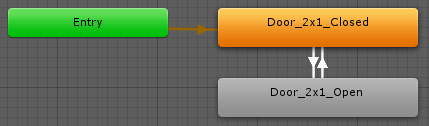
\includegraphics[width=0.5\linewidth]{pics/animation_example.PNG}
 \captionof{figure}[Beispiel für einen \textit{Animator}]{Beispiel für den Zustandsautomaten eines \textit{Animators} für eine Tür.}
	\label{fig:animator_example}
\end{figure}

Animationen an sich haben soweit noch keinen Effekt auf eine laufende Spielszene. Hierzu muss zu dem Spielobjekt, welches animiert werden soll, ein sogenannter \textit{Animator} \cite{Unity_Doc_Animator} als Komponente hinzugefügt werden. Dieser definiert über einen Zustandsautomaten die Übergänge zwischen den einzelnen Animationen sowie die Zeitpunkte, wann diese ausgelöst werden, wie in Abbildung \ref{fig:animator_example} anhand einer Türanimation zu sehen ist. "`Door\_2x1\_Open"' und "`Door\_2x1\_Close"' sind im Beispiel die entsprechenden Einzelanimationen zum Öffnen und Schließen der Tür. Die Übergänge zwischen den einzelnen Zuständen können entweder zeitlich oder durch Setzen entsprechender selbst definierter Variablen ausgelöst werden. Jede Animation wird beim Zustandsübergang zu dieser einmal abgespielt und, sofern dementsprechend definiert, bis zum nächsten Übergang wiederholt.

Für statische Elemente der Benutzeroberfläche wird als Eltern-Spielobjekt zumeist ein \textit{Canvas} \cite{Unity_Doc_Canvas} eingesetzt. Dieser erstreckt sich in der Regel über den gesamten Bildschirm und dient als Anker für alle Kindelemente. So können Objekte für die Benutzeroberfläche zum Beispiel relativ zum \textit{Canvas} in der rechten oberen Ecke platziert werden. Dies gewährleistet, dass die Oberflächenelemente dynamisch mit der Bildschirmgröße skalieren und entsprechend positioniert werden, sodass die Oberfläche unabhängig von der Bildschirmauflösung ist.